%\newpage
\section{Experiments}
\label{sec:experiments}
\subsection{Dataset and Experimental Setting}
\subsubsection{Dataset}
\label{subsec:Dataset}
In our research center, at USC's IMSC, with our partnership with Los Angeles Metropolitan Transportation Authority (LA Metro), we maintain a big transportation data warehouse that fuses and analyzes a very large-scale and high-resolution (both spatial and temporal) traffic sensor data from different transportation authorities in Southern California, including California Department of Transportation (Caltrans), Los Angeles Department of Transportation (LADOT), California Highway Patrol (CHP), Long Beach Transit (LBT).  This data set includes both inventory and real-time data with update rate as high as every 30 seconds for freeway and arterial traffic sensors (9300 loop-detectors) covering more than 3500 miles, incidents  such as accidents, traffic hazards and road closures reported (approximately 400 per day) by LAPD and CHP, and ramp meters. We have been continuously collecting and archiving aforementioned datasets for the past three years. We use this real-world dataset to model and evaluate our techniques. To generate time dependent  travel times we spatially and temporally aggregate traffic sensor data by assigning interpolation points for each 5 minutes during a year that depict the travel-times on the segments of Los Angeles road network with 304,162 edges. Based on our observation, all roads are fairly un-congested between 9:00pm and 6:00am, and hence we assume static edge weights between those times. More detailed information regarding the dataset can be found in \cite{Jagadish14}.

\subsubsection{Experimental Setting}
All experiments were conducted on an Intel(R) Core(TM)2 Duo 3.16GHz PC running on Microsoft Windows 7. Methods were implemented in Java.

Predicting travel times in a rather static road network (with only marginal changes in the link travel times) is not very challenging and usually does not require a probabilistic prediction. For this reason we focused on rush hour times which imply more uncertainty and thus a much harder scenario for prediction. If not mentioned otherwise we used 8:00am, 9:00am, 4:00pm, 5:00pm and 6:00pm during the weekdays. These times were considered as the \textit{start time}, i.e. the time at which the user starts his route. According to the results from \cite{Pan12} and our own observations, traffic patterns are quite equivalent across weekdays. Consequently, we did not differentiate between predictions for different weekdays. This means for each start time, we consider data of 260 days (5 days per week, 52 week per year). \\
In our evaluation process, we used the k-fold cross validation (k=5) method to divide our data into test (test days) and training (training days) sets. In each fold, for each start time and each test day we investigated the following:
\begin{itemize}
  \item We used the data of the training days with one of our techniques to build a model for predicting the travel time of a link (\textbackslash route) at a specific start time. In case the \textit{current situation} is required for building the model, we can fetch it from the dataset.
  \item For the specific test day and start time, we find the \textit{actual} travel time over the link (\textbackslash route) from the dataset.
\end{itemize}
Both of these outcomes are then used to compute a CRPS score as defined in Section \ref{sec:evaluate}, which is then averaged over all folds and trials. For all discrete models we discretize the time into 1 second intervals.

\subsection{Probabilistic Link Travel Time Prediction}
\label{subsec:pltt_prediction}
In our first set of experiments we evaluate the prediction quality of the following three proposed approaches:
\begin{itemize}
  \item HP: Prediction purely based on historical data as described in \cref{subsec:historical}.
  \item LI: Prediction based on linear interpolation between the current situation and the prediction based on historical data as discussed in \cref{subsec:LI}.
  \item SH: Prediction based on historical data with behavior similar to the current situation as proposed in \cref{subsec:SH}.
\end{itemize}

We tested all techniques over 50 links which are chosen randomly from all around the road network explained in \cref{subsec:Dataset}. The links we chose for these experiments are ~1 mile long and all are on highways. The link selection process was such that we had 6-8 links from each major highway in the L.A. metropolitan area. The farther an event is in the future, the harder it gets to predict it. For each start time during the experiments we use different prediction times varying from 0 minutes up to 120 minutes.

\begin{figure}[h]
	\centering
	\subfigure[Different Prediction Times] {
		\label{fig:HP1}
		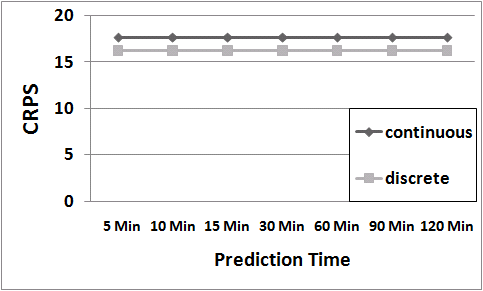
\includegraphics[width = 0.6\columnwidth]{figures/Links_Historic.png}
	}
	\subfigure[Different Start Times]{
		\label{fig:HP2}
		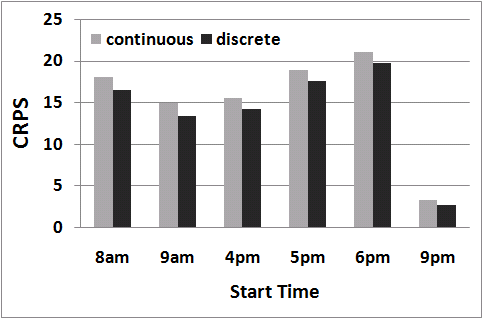
\includegraphics[width = 0.6\columnwidth]{figures/Links_Historic_TOD.png}
	}
	\caption{CRPS Score for HP Approach}\label{fig:HP}
\end{figure}

With the HP approach, we only consider historic data. This means that if we use 8:00am as the \textit{start time}, we consider the travel times at 8:00am across the training days and build the model distribution. Subsequently, we retrieve the actual travel time at 8:00am for each test day and compare it with the model. Since the historic approach is based on historical data only and does not depend on current situation (\textit{query time}), it is consequently independent form the \textit{prediction offset} (\cref{fig:HP1}). \cref{fig:HP2} shows results of the HP approach for different start times in the day with two implications. First, different times of the day are differently hard to predict. In particular the selected standard start times yield much higher CRPS compared to 9:00pm, where there is not too much traffic on the road network and thus not a lot of uncertainty in the prediction.  Second, it shows that the continuous and discrete representation performs rather equivalent. The small difference between the discrete and the continuous case can be explained by the fact that a discrete representation copes better with non-normally distributed link travel times. However, it is important to note that the CRPS of the discrete representation is very sensitive to the discretization interval of the time, i.e., a large discretization interval leads to a larger value of the CRPS and hence not directly comparable to the CRPS of the continuous representation.

Since the results for continuous and discrete link travel times are rather equivalent, for the remainder of the experiments on link travel times we only present results for discrete representation of travel times.

\begin{figure}[h]
    \centering
    \subfigure[Different time horizons]{
        \label{fig:LI1}
        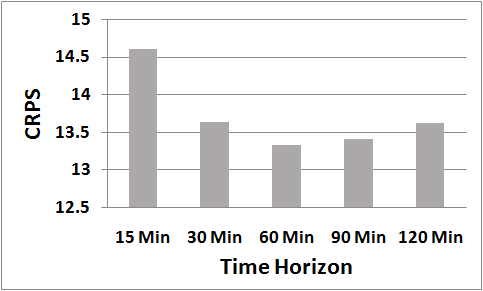
\includegraphics[width = 0.6\columnwidth]{figures/Links_Interpolated_TimeHorizon.png}
    }
    \subfigure[Different values of $\theta$]{
        \label{fig:LI2}
        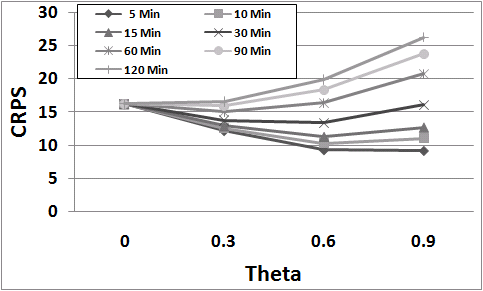
\includegraphics[width = 0.6\columnwidth]{figures/Links_Interpolated_Theta.png}
    }
    \caption{Experiments for the LI approach}\label{fig:LI}
\end{figure}



With regards to the LI approach, we studied the accuracy of the model for
different time horizons $\tau$, ranging from 15 minutes up to 120 minutes. The
results in \cref{fig:LI1} are averaged over all \textit{prediction times} and
clearly show neither of these extremes should be chosen, but rather a good
choice of the time horizon is somewhere in between (i.e., around 60 minutes).
These results are backed up by the experiments shown in \cref{fig:LI2}. In the
LI approach, we eventually use the time horizon to compute $\theta$ as the
weight of the current situation versus historic data. In \cref{fig:LI2} we
directly assign different values to $\theta$. If increasing $\theta$ yields
better results, it means assigning more weight to the current situation is
beneficial and vice versa. \cref{fig:LI2} shows that for prediction times
greater or equal to 60 minutes, increasing $\theta$ results in higher CRPS
scores. Hence we can say, the current situation has no positive influence on the
prediction after 60 minutes, which is the definition of the time horizon
parameter in \cref{subsec:LI}. We use the results in \cref{fig:LI} to conclude
that an optimal time horizon in the Linear Interpolation technique is 60
minutes. Let us note that this is an insightful finding in itself. This result
suggests, that the traffic ``forgets'' its condition an hour ago.

\begin{figure}
	\centering
	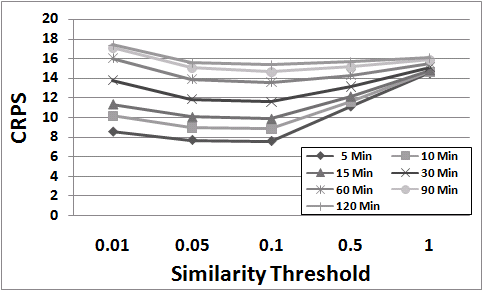
\includegraphics[width = 0.6\columnwidth]{figures/Links_Filtered.png}
	\caption{CRPS Score for SH Approach}\label{fig:SH}
\end{figure}

In the next set of experiments, we evaluate the accuracy of the SH approach. As explained in \cref{subsec:SH}, SH only considers the historical data similar to the current situation. We also defined similarity by the parameter $\lambda$ in \cref{subsec:SH}. We assign different values to $\lambda$ and compare the results.\cref{fig:SH} shows the results. Like LI, SH predicts the near future more accurate than the far future since it is taking the current situation into account. For smaller values of $\lambda$ (e.g., 0.01 \& 0.05) the predictions yield generally higher CRPS. The reason for this behavior is that only very few measurements of the training data meet the similarity
requirement and thus the prediction is based on a possibly non-representative sample. Therefore, as the similarity threshold increases, our model gets more realistic and the results get better. On the other hand, if the similarity
threshold is too loose, data that is not similar to the test day is considered in generating the model, which results in less accurate models.

\begin{figure}[h]
	\centering
	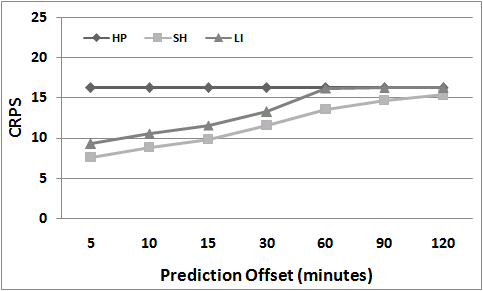
\includegraphics[width = 0.6\columnwidth]{figures/Links_Best.png}
	\caption{CRPS Scores for HP, LI and SH}\label{fig:all_results}
\end{figure}

Finally, we compared the three approaches to each other, using the best setting for the corresponding parameters ($\tau = 60$ minutes and $\lambda = 0.1$). The results are illustrated in \cref{fig:all_results}. Clearly, LI and SH are able to predict the near future more accurately than the farther future, whereas HP is independent from the \textit{prediction offset}. As expected, when $\tau = 60$, for prediction times greater than 60 minutes, LI and HP give the same model. In the following experiments we will use the results of \cref{fig:all_results} to show the important fact that the accuracy of all algorithms proposed to compute a pmf for a route, directly depends on how accurate the probabilistic link travel times are estimated on such route.

